%%%%%%%%%%%%%%%%%%%%%%%%%%%%%%%%%%%%%%%%%
% Masters/Doctoral Thesis 
% LaTeX Template
% Version 2.4 (22/11/16)
%
% This template has been downloaded from:
% http://www.LaTeXTemplates.com
%
% Version 2.x major modifications by:
% Vel (vel@latextemplates.com)
%
% This template is based on a template by:
% Steve Gunn (http://users.ecs.soton.ac.uk/srg/softwaretools/document/templates/)
% Sunil Patel (http://www.sunilpatel.co.uk/thesis-template/)
%
% Template license:
% CC BY-NC-SA 3.0 (http://creativecommons.org/licenses/by-nc-sa/3.0/)
%
%%%%%%%%%%%%%%%%%%%%%%%%%%%%%%%%%%%%%%%%%

%----------------------------------------------------------------------------------------
%	PACKAGES AND OTHER DOCUMENT CONFIGURATIONS
%----------------------------------------------------------------------------------------

\documentclass[
11pt, % The default document font size, options: 10pt, 11pt, 12pt
%oneside, % Two side (alternating margins) for binding by default, uncomment to switch to one side
english, % ngerman for German
singlespacing, % Single line spacing, alternatives: onehalfspacing or doublespacing
%draft, % Uncomment to enable draft mode (no pictures, no links, overfull hboxes indicated)
%nolistspacing, % If the document is onehalfspacing or doublespacing, uncomment this to set spacing in lists to single
%liststotoc, % Uncomment to add the list of figures/tables/etc to the table of contents
%toctotoc, % Uncomment to add the main table of contents to the table of contents
%parskip, % Uncomment to add space between paragraphs
%nohyperref, % Uncomment to not load the hyperref package
headsepline, % Uncomment to get a line under the header
%chapterinoneline, % Uncomment to place the chapter title next to the number on one line
%consistentlayout, % Uncomment to change the layout of the declaration, abstract and acknowledgements pages to match the default layout
]{MastersDoctoralThesis} % The class file specifying the document structure

\usepackage[utf8]{inputenc} % Required for inputting international characters
\usepackage[T1]{fontenc} % Output font encoding for international characters

\usepackage{palatino} % Use the Palatino font by default

\usepackage[backend=bibtex,style=authoryear,natbib=true]{biblatex} % Use the bibtex backend with the authoryear citation style (which resembles APA)

\addbibresource{example.bib} % The filename of the bibliography

\usepackage[autostyle=true]{csquotes} % Required to generate language-dependent quotes in the bibliography

\usepackage{float} % In order to use the [H] option for figure alignment

\usepackage{fancyvrb} % keep tabs in verbatim sections, see: https://tex.stackexchange.com/questions/231083/how-to-stop-verbatim-from-converting-tabs-to-spaces

%----------------------------------------------------------------------------------------
%	MARGIN SETTINGS
%----------------------------------------------------------------------------------------

\geometry{
	paper=a4paper, % Change to letterpaper for US letter
	inner=2.5cm, % Inner margin
	outer=3.8cm, % Outer margin
	bindingoffset=.5cm, % Binding offset
	top=1.5cm, % Top margin
	bottom=1.5cm, % Bottom margin
	%showframe, % Uncomment to show how the type block is set on the page
}

%----------------------------------------------------------------------------------------
%	THESIS INFORMATION
%----------------------------------------------------------------------------------------
\title{Doctoral Thesis}
\thesistitle[0, 0]{Multimesh Methods for Data Visualization and Finite Element Analysis} % Your thesis title, this is used in the title and abstract, print it elsewhere with \ttitle
\supervisor{Dr. James \textsc{Smith}} % Your supervisor's name, this is used in the title page, print it elsewhere with \supname
\examiner{} % Your examiner's name, this is not currently used anywhere in the template, print it elsewhere with \examname
\degree{Doctor of Philosophy} % Your degree name, this is used in the title page and abstract, print it elsewhere with \degreename
\author{John \textsc{Smith}} % Your name, this is used in the title page and abstract, print it elsewhere with \authorname
\addresses{} % Your address, this is not currently used anywhere in the template, print it elsewhere with \addressname

\subject{Biological Sciences} % Your subject area, this is not currently used anywhere in the template, print it elsewhere with \subjectname
\keywords{} % Keywords for your thesis, this is not currently used anywhere in the template, print it elsewhere with \keywordnames
\university{\href{http://www.university.com}{University Name}} % Your university's name and URL, this is used in the title page and abstract, print it elsewhere with \univname
\department{\href{http://department.university.com}{Department or School Name}} % Your department's name and URL, this is used in the title page and abstract, print it elsewhere with \deptname
\group{\href{http://researchgroup.university.com}{Research Group Name}} % Your research group's name and URL, this is used in the title page, print it elsewhere with \groupname
\faculty{\href{http://faculty.university.com}{Faculty Name}} % Your faculty's name and URL, this is used in the title page and abstract, print it elsewhere with \facname

\AtBeginDocument{
\hypersetup{pdftitle=\ttitle} % Set the PDF's title to your title
\hypersetup{pdfauthor=\authorname} % Set the PDF's author to your name
\hypersetup{pdfkeywords=\keywordnames} % Set the PDF's keywords to your keywords
}

\begin{document}

\frontmatter % Use roman page numbering style (i, ii, iii, iv...) for the pre-content pages

\pagestyle{plain} % Default to the plain heading style until the thesis style is called for the body content

%----------------------------------------------------------------------------------------
%	TITLE PAGE
%----------------------------------------------------------------------------------------

\begin{titlepage}
\begin{center}

\vspace*{.06\textheight}
{\scshape\LARGE \univname\par}\vspace{1.5cm} % University name
\textsc{\Large Doctoral Thesis}\\[0.5cm] % Thesis type

\HRule \\[0.4cm] % Horizontal line
{\huge \bfseries \ttitle\par}\vspace{0.4cm} % Thesis title
\HRule \\[1.5cm] % Horizontal line
 
\begin{minipage}[t]{0.4\textwidth}
\begin{flushleft} \large
\emph{Author:}\\
\href{http://www.johnsmith.com}{\authorname} % Author name - remove the \href bracket to remove the link
\end{flushleft}
\end{minipage}
\begin{minipage}[t]{0.4\textwidth}
\begin{flushright} \large
\emph{Supervisor:} \\
\href{http://www.jamessmith.com}{\supname} % Supervisor name - remove the \href bracket to remove the link  
\end{flushright}
\end{minipage}\\[3cm]
 
\vfill

\large \textit{A thesis submitted in fulfillment of the requirements\\ for the degree of \degreename}\\[0.3cm] % University requirement text
\textit{in the}\\[0.4cm]
\groupname\\\deptname\\[2cm] % Research group name and department name
 
\vfill

{\large \today}\\[4cm] % Date
%\includegraphics{Logo} % University/department logo - uncomment to place it
 
\vfill
\end{center}
\end{titlepage}

%----------------------------------------------------------------------------------------
%	DECLARATION PAGE
%----------------------------------------------------------------------------------------

\begin{declaration}
\addchaptertocentry{\authorshipname} % Add the declaration to the table of contents
\noindent I, \authorname, declare that this thesis titled, \enquote{\ttitle} and the work presented in it are my own. I confirm that:

\begin{itemize} 
\item This work was done wholly or mainly while in candidature for a research degree at this University.
\item Where any part of this thesis has previously been submitted for a degree or any other qualification at this University or any other institution, this has been clearly stated.
\item Where I have consulted the published work of others, this is always clearly attributed.
\item Where I have quoted from the work of others, the source is always given. With the exception of such quotations, this thesis is entirely my own work.
\item I have acknowledged all main sources of help.
\item Where the thesis is based on work done by myself jointly with others, I have made clear exactly what was done by others and what I have contributed myself.\\
\end{itemize}
 
\noindent Signed:\\
\rule[0.5em]{25em}{0.5pt} % This prints a line for the signature
 
\noindent Date:\\
\rule[0.5em]{25em}{0.5pt} % This prints a line to write the date
\end{declaration}

\cleardoublepage

%----------------------------------------------------------------------------------------
%	QUOTATION PAGE
%----------------------------------------------------------------------------------------

\vspace*{0.2\textheight}

\noindent\enquote{\itshape Thanks to my solid academic training, today I can write hundreds of words on virtually any topic without possessing a shred of information, which is how I got a good job in journalism.}\bigbreak

\hfill Dave Barry

%----------------------------------------------------------------------------------------
%	ABSTRACT PAGE
%----------------------------------------------------------------------------------------

\begin{abstract}
\addchaptertocentry{\abstractname} % Add the abstract to the table of contents
The Thesis Abstract is written here (and usually kept to just this page). The page is kept centered vertically so can expand into the blank space above the title too\ldots
\end{abstract}

%----------------------------------------------------------------------------------------
%	ACKNOWLEDGEMENTS
%----------------------------------------------------------------------------------------

\begin{acknowledgements}
\addchaptertocentry{\acknowledgementname} % Add the acknowledgements to the table of contents
The acknowledgments and the people to thank go here, don't forget to include your project advisor\ldots
\end{acknowledgements}

%----------------------------------------------------------------------------------------
%	LIST OF CONTENTS/FIGURES/TABLES PAGES
%----------------------------------------------------------------------------------------

\tableofcontents % Prints the main table of contents

\listoffigures % Prints the list of figures

\listoftables % Prints the list of tables

%----------------------------------------------------------------------------------------
%	ABBREVIATIONS
%----------------------------------------------------------------------------------------

\begin{abbreviations}{ll} % Include a list of abbreviations (a table of two columns)

\textbf{LAH} & \textbf{L}ist \textbf{A}bbreviations \textbf{H}ere\\
\textbf{WSF} & \textbf{W}hat (it) \textbf{S}tands \textbf{F}or\\

\end{abbreviations}

%----------------------------------------------------------------------------------------
%	PHYSICAL CONSTANTS/OTHER DEFINITIONS
%----------------------------------------------------------------------------------------

\begin{constants}{lr@{${}={}$}l} % The list of physical constants is a three column table

% The \SI{}{} command is provided by the siunitx package, see its documentation for instructions on how to use it

Speed of Light & $c_{0}$ & \SI{2.99792458e8}{\meter\per\second} (exact)\\
%Constant Name & $Symbol$ & $Constant Value$ with units\\

\end{constants}

%----------------------------------------------------------------------------------------
%	SYMBOLS
%----------------------------------------------------------------------------------------

\begin{symbols}{lll} % Include a list of Symbols (a three column table)

$a$ & distance & \si{\meter} \\
$P$ & power & \si{\watt} (\si{\joule\per\second}) \\
%Symbol & Name & Unit \\

\addlinespace % Gap to separate the Roman symbols from the Greek

$\omega$ & angular frequency & \si{\radian} \\

\end{symbols}

%----------------------------------------------------------------------------------------
%	DEDICATION
%----------------------------------------------------------------------------------------

\dedicatory{For/Dedicated to/To my\ldots} 

%----------------------------------------------------------------------------------------
%	THESIS CONTENT - CHAPTERS
%----------------------------------------------------------------------------------------

\mainmatter % Begin numeric (1,2,3...) page numbering

\pagestyle{thesis} % Return the page headers back to the "thesis" style

% Include the chapters of the thesis as separate files from the Chapters folder
% Uncomment the lines as you write the chapters

\chapter{Introduction}
\label{chapter:introduction}

The research work presented in this thesis has set ambitious goal to redesign the whole well established process of data management in Finite element analysis software. It also proposes efficient methods to visualize finite element meshes and the results from the complex finite element analyses.

Finite Element Analysis (FEA) is the term describing the entire process of modeling the physical system using the Finite Element Method (FEM). FEA consists of model generation, meshing, attribute assignment, solution, and post-processing. With the ongoing desire to solve more complex systems with better and better precision, an analysis has to process enormous amount of data in each of its phases. Traditional unstructured file-based representation of the mesh, input parameters, and the results from the solution is the bottleneck of the entire process. It lacks the scalability and complicates the development of the tools for engineers that are either preparing the input to the FEM, or interpreting the output from the FEM.

The solution of large-scale Finite element analysis itself can be parallelized and calculated in reasonable time on high-performance computing clusters. Nevertheless, in the end the results are transfered over network and post-processed on an ordinary personal computer. Another concern is the colaboration and sharing of the model and the results between engineers and researchers. All these limitation of the standard file-based approach lead to re-think the entire process of data management in FEA. The focus of the thesis is mainly on the post-processing of the results, and the way the results are stored, transfered, and visualized. However, the storage format for the results was designed with the whole picture in mind and there is proposed database-centric environment for complete FEA data management.

As an motivation example can serve analysis of reactor vessels in nuclear power plants which is used in the process of prolongation of their service life. The vessels are approximately 40 years old and detailed thermo-hydro-mechanical analysis has to be performed. Usually, two-dimensional axisymmetric or fully three-dimensional models are considered and it means hundreds of thousands degrees of freedom are used. The number of time steps is between 10,000 and 15,000. The output files contain displacements, strain and stress components, temperature, relative humidity (or moisture content) and several internal parameters (e.g. creep strains, damage parameter, etc.) in all time steps. The output files with size in the order of gigabytes are generated. More details can be found in \cite{XXX-1,XXX-2}.

\begin{figure}[H]
\centering

\includegraphics[width=\textwidth]{figures/chapter-introduction/motivation-example}
\decoRule
\caption[TODO: ]{TODO: Motivation example visualization}
\label{fig:motivation-example}
\end{figure}

The thesis is structured in the following manner. Chapter \ref{chapter:related-work} gives a brief revision of related work performed in FEA data management, file formats, data compression, and post-processing of the results. Chapter \ref{chapter:data-management} deals with the alternative to file-based data management. Section \ref{sec:system-architecture} contains proposal of relational database model that connects all parts of Finite element analysis including geometry, model attributes, and simulation results, providing query interface and remote access over the Internet. Section \ref{sec:storage-format} describes details of new data format. Section \ref{sec:postprocessing} presents design of the postprocessor that is built on top of the data management system. Chapter \ref{chapter-implementation} summarizes interesting technical details and challenges that arose during implementation of the management system and post-processor. Chapter \ref{chapter:overall-results} evaluates the implementation of the tools that are based on the new storage format and contains comparison to the traditional data formats. Chapter \ref{chapter:conclusion} concludes the thesis with final remarks, benefits and weaknesses of the chosen solution, and possible future work.

%----------------------------------------------------------------------------------------
%	SECTION Concepts
%----------------------------------------------------------------------------------------

\section{Concepts}

Here follows a summary of basic terms and concepts the thesis is based on.

\paragraph{Finite Element Method (FEM).} FEM is a numerical method for solving problems of engineering and physics. Typical areas include structural analysis, heat transfer, fluid flow, and electromagnetics. The analytical solution of these problems generally require the solution to boundary value problems for partial differential equations. The finite element method formulation of the problem results in a system of algebraic equations. The method yields approximate values of the unknowns at discrete number of points over the domain \cite{XXX}. To solve the problem, it subdivides a large problem domain into smaller, simpler parts that are called finite elements. This process is called the mesh generation \cite{XXX}. The simple equations that model these finite elements are then assembled into a larger system of equations that models the entire problem. FEM then uses variational methods from the calculus of variations to approximate a solution by minimizing an associated error function \cite{XXX}. The focus of this thesis is exclusively on the data management problems in the context of FEM-based simulations, not the simulations themselves.

% TODO: do predchoziho odstavce vlozit vysvetleni gaussovych/integracnich bodu

\paragraph{Finite Element Analysis (FEA).} Various data creation and modification tasks precede and follow the actual numerical solution of the boundary value problem using FEM. This whole process is called \textbf{Finite element analysis} and consists of several distinct phases. The basic phases of a FEA depicted in Figure \ref{fig:FEA-phases} are\footnote{This is a quite simplified description of the FEA process as the results from one simulation are then sometimes used as an input for other simulations. Preliminary results of the simulation can also be post-processed continualy during the calculation phase to monitor the convergence of the iterative methods. Another case represent the iso-parametric representation of finite elements \cite{XXX} and NURBS-enhanced FEM \cite{XXX}. These new approches are somewhat bridging the mesh generation phase as the curves describing the geometry are used also as the base functions of the finite elements.}:

\begin{enumerate}
    \item \textbf{Model creation} phase describes geometry of the domain, typically by defining boundaries of the domain using parametric surfaces like Bézier patches or Non-Uniform Rational Bézier-Splines (NURBS) \cite{XXX} in a CAD (Computer Aided Design) tool.
    \item \textbf{Attribute definition and assignment} specifies properties of the model, i.e. material properties of volumes, initial and boundary conditions for the solution.
    \item \textbf{Mesh generation} decomposes the geometry of the model into simple shapes (triangles or quadrilaterals) or voxels like tetrahedra or bricks that fill the volume. This is often only an approximation of the orignal domain, because it is not possible for these simple shapes to fill the complex domain completely without gaps.
    \item \textbf{FEM solution} uses the equations describing the problem, model discretization, and attributes to simulate the system's behavior. Often, the process is parametric either in geometry, or in assigned attributes. Simulation then produces multiple sets of output data, each for different configuration.
    \item \textbf{Post-processing} of results is examination of the output by engineer or scientist, who is seeking the features and trends in data using the visualization tool.
\end{enumerate}

\begin{figure}[H]
    \centering
    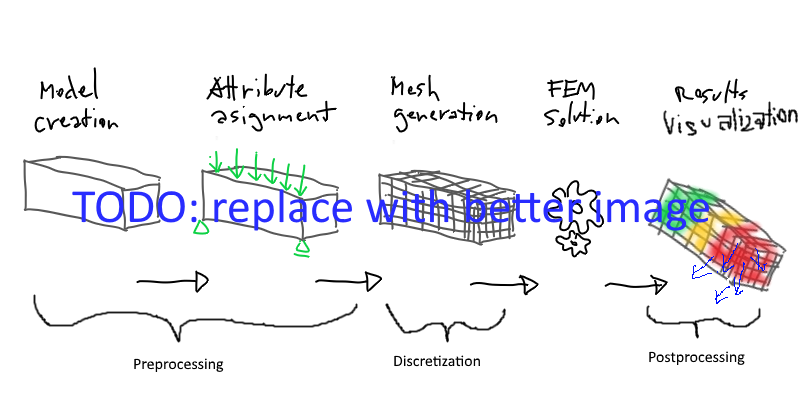
\includegraphics[width=\textwidth]{figures/chapter-introduction/FEA-phases}
    \decoRule
    \caption[TODO: ]{TODO: FEA phases}
    \label{fig:FEA-phases}
\end{figure}

Visualization tools are used to explore and analyse the data during all the phases. However, the vast majority of discussion about FEA focuses on the solution phase only. This makes sense as the solution phase consumes the largest portion of the computer time. But the solution phase itself consumes the insignificant amount of people-time. The majority of people's time is spent in pre-processing and post-processing of complex models. This fact seems to be overlooked and is one of the motivations for research work presented in this thesis.

\paragraph{FEM results.} Results from FEM are scalar, vector, or tensor fields represented by discrete values. Some results are stored in nodes of the mesh, such as vectors of nodal displacements. Other results are stored typically in Gauss points (i.e. integration points) on finite elements. There are two similar sets of results. One is generated by a non-linear algorithms, where several incremental steps are stored and the other is generated by time integration, where results in particular time steps are stored. These results are represented as dense tabular values of basic types, usually double-precision floating-point numbers (8 bytes each). For example, a 3D material stress calculation of the domain discretized by tetrahedral elements with quadratic approximation yields 12 values for the stress and strain tensors in each Gauss points. There are 11 Gauss points in each element. If 100 time samples are taken, the size of the solution output is $100 \times 12 \times 11 \times 8 \approx 100$ kilobytes per single (!) element. The number of finite elements depends on (1) the resolution of the discretization, (2) the geometric complexity of the model, and (3) the desired accuracy of output. In practice, fine discretizations of the problem domain contain millions of elements.

Current FEA software packages store the results either sequentially in formatted \textit{ASCII or binary files} ordered by time steps, or use more sophisticated \textit{database}\footnote{The term database is used here to describe any structured storage beyond a simple file store.} systems to preserve the links between the input model and the simulation results. Either way, the size of output data is very large for non-trivial analyses, which puts pressure on storage capacity, transfer times over the network, and memory consumption of postprocessing tools.

\paragraph{Data compression.} A compression method can be lossy or lossless. Lossless methods reduce information by identifying and eliminating statistical redundancy in data and are therefore able to fully reconstruct original data from its compressed form. Lossy methods, on the other hand, reduce the size by removing less important information in data and are thus producing only the approximation of original data.

\paragraph{Approximation error.} Compression methods usually yield approximated data. In the following text, the term approximation error denotes an error resulted from compression, i.e. difference between original results of FEM analysis and their compressed form. It should not be confused with the error of the Finite Element Method itself that yields approximate solution to mathematical problems used to model physical reality. There are defined several error metrics in the text (Section \ref{sec:error-estimation}) that are used to measure the approximation error.

% TODO: vysvetlit, proc pouzivam pojem Multi-mesh (Multigrid byla inspirace)

% TODO: pridat dalsi pojmy/hesla, ktera potrebuji vysvetlit. Tato kapitola by mela fungovat jako slovnicek pojmu

%----------------------------------------------------------------------------------------
%	SECTION Aims
%----------------------------------------------------------------------------------------

\section{Aims} % or Goal of the thesis

\begin{itemize}
    \item The main goal of the research work is to develop a new storage format that supports compression of results, and to outline the transition to a new post-processor that can read and visualize the compressed data in the new storage format. There is understandable resistance against invention of new data formats in the area of information technology. A new format leads to fragmentation of user base and compatibility issues. Conversion tools need to be created and maintained. There should be a strong motivation for introduction of a new format. However, there is no standard format for representation of results from FEM. Each software package uses proprietary format with syntax suitable for its internal implementation. There is also lack of support for compression methods that fit the character of FEM results. Standard file-based format does not allow for querying of specific information without the need to parse through the complete set of results. Chapter \ref{chapter:related-work} contains discussion about the existing formats in more detail and Chapter \ref{chapter:data-management} describes the proposed format.
    \item In addition, several suitable compression methods are proposed. Singular Value Decomposition (SVD) (Chapter \ref{chapter:SVD}) is the most promising method used for compression of results in this research. Other methods, that are investigated, include Wavelet transform (\ref{XXX}) and approximation of discrete values by continuous polynomial functions (Chapter \ref{chapter:approximation}).
    \item Finally, the product of this research is the implementation of two postprocessors. The first is a standard desktop postprocessor that is based on existing software and should present the way of transition from the convential file-based formats to the proposed structured database format utilizing compression. The second postprocessor is a web-based thin client intended to present advantages of the proposed format when incorporated into a complex FEA running on a remote server. Chapter \ref{chapter-implementation} summarizes implementation details.
\end{itemize}

%----------------------------------------------------------------------------------------
%	SECTION Challenges
%----------------------------------------------------------------------------------------

\section{Challenges}

Main challenge is a design of universal format that can hold the results from any FEM analysis. Results are composed of scalars, vectors, or tensors. Each field with different number of components. The results can be located on nodes or integration points. There may be a requirement to extrapolate the results from integration points to element nodes. There are different extrapolation strategies. Mesh can be different for each time step (e.g. in case of simulating the construction stages). Mesh can contain 1D, 2D, or 3D elements. Each of different type and approximation. Results from 3D simulations can be visualized on the surface of the mesh, in form of cross-sections or iso-areas, or as a vector field. The storage format should support efficient generation of all these views of results.

Finite element solution and post-processing of results can be sometimes done on different computers. Complex FEA solution phase runs on a supercomputer or a performant cluster of workstations, but the results are post-processed on common personal computer that has significantly less memory available. Typical personal computer has 8 to 16 GB of RAM available while the size of results can be in order of tens to hunderds of gigabytes. Also, the data to postprocess have to be first transfered over the corporate network or the Internet. These conditions indicate the need for partitioning of data into smaller chunks and/or compression of data.

The goal of compression methods is a significant reduction in size while preserving the quality (keeping the approximation error low). Unlike with image compression methods where the main aspect is the human perception of the reconstructed image the compression of FEM results should be able to guarantee the matematical acuracy of the approximations and the user should be able to specify a desired value of the approximation error. Another concern is the computation complexity of the compression algorithm. The compression will be performed only once after the solution phase is complete. The computational time should be order of magnitude lower compared to the solution phase. Decompression (reconstruction of the original data) should be very fast as it is supposed to be performed every time the data are post-processed on the end device, which can be ordinary PC or even mobile device. The ability to create animations should also be taken into account.

Other kind of challenge is to provide a data management system that will connect all the FEA phases, i.e. to provide links between the geometric model, the mesh entities, and the output values. A project typically encompasses multiple simulations, each with different input or solver parameters. Multiple users are usually involved in the project and the system should help them to cooperate during the preparation of the input and allow to share the output of the analysis. All these aspects influence the design of the data management system.

% TODO: Pridat dalsi vyzvy a namety. Napr.:
% Slo by propojit vypocet a zpracovani vysledku? Zminit multigrid.
% Co takhle nejak zohledit chybu aproximace FEMu, zohlednit ji pri kompresi a prezentovat ji uzivateli?

\chapter{Related work}
\label{chapter:related-work}

This chapter gives a brief revision of related research work that deals with visualization of finite element meshes and results from FEM, file formats used for representation of FEM data, compression methods, and FEA data management.

% TODO: State of the art and discussion about related work in the area of FEM results post-processing, storage formats, and cloud-based FEA.

\section{Data compression and visualization}
% Vrstva je koncept, ktery se vyskytuje i u jinych postprocessoru (napr. Simscale)

mesh compression:

surface mesh visualization (refinement/progressive meshes):
\cite{Gudukbay2002}
\cite{Vasa2011}
\cite{Alliez2001}
\cite{Maglo2012}
\cite{Valette2004}

\cite{Hoppe1996}

% Quite surprisingly, most of the existing algorithms mainly use only general compression techniques, such as entropy coding, quantisation, PCA or wavelet decomposition, while the inherent geometrical properties of the compressed surface remain unexploited. In this paper we focus on geometry specific optimisation: we extend the PCA-based dynamic mesh compression by optimising the order in which the mesh is traversed.

volumetric mesh visualization:
\cite{Ueng2004}, \cite{Robaina2010}

Iso geometric analysis + post-processing
\cite{Stahl2017}

3D graphics on the web:
\cite{Evans2014}
\newline
\cite{Hoppe1998}, \cite{Limper2013}, \cite{Maglo2012}, \cite{Lavoue2013}, \cite{Valette2009}, \cite{Charland2011}, \cite{Behr2012}, \cite{OpenCTM2010}, \cite{Mouton2011}, \cite{Marion2012}, \cite{Alliez2005}

% Data compression is a very wide area - image compression is related, fem data compression se nedela, VTK sice podpoduje kompresi ale obycejnou zip?
Image compression methods:
\cite{Lui2001}
\cite{Watson1994}

\section{File formats}
% univerzalni formaty pro vstupni geometrii:
IGES (Initial Graphics Exchange Specification) \cite{Groton2006}, STEP (STandard for the Exchange of Product model data) \cite{Pratt2001}

% http://blog.grabcad.com/blog/2014/10/14/get-over-iges/

% BREP, STL, ... formats; VRML

% OpenCASCADE
\cite{OpenCASCADE}

% Abaqus
\cite{Abaqus}

\cite{McHenry2008}  presents about 140 file formats for representation of 3D models...


% VTK format podporuje kompresi, ale bez znalosti obsahu dat. Pouze nejakou ZIP kompresi ci co. Neni to tak efektivni. Kazdy casovy krok ulozeny zvlast. Ale umi ukladat v ascii i binarne (base64 kodovani)



% pro vysledky: proprietary formats, VTK open source - used in scientific reasearch mainly, Gmsh - open, GiD - proprietary, Abaqus, ...

% zatimco pro reprezentaci geometrickeho modelu existuje spousta standardizovanych formatu, pro reprezentaci vysledku neexistuje otevreny univerzalni format podporujici kompresi. snad jen s vyjimkou VTK, ale ten ma sve nedostatky

% https://scicomp.stackexchange.com/questions/23882/what-is-a-common-file-data-format-for-a-mesh-for-fem

VTK: \cite{VTK2015}
Gmsh: \cite{Geuzaine2009}
GiD: \cite{GiDPostProcess}
Abaqus: 
\newline
\cite{Ivanyi2012}

% TODO: prozkoumat dalsi formaty pro ulozeni vysledku (vetsinou asi proprietarni, zadny standard neexistuje?)

\section{Web-based data management}

% citovat papery
\cite{Ari2013}
\cite{Yu2010}
\cite{Peng2003}
\cite{Heber2007I}
\cite{Heber2007II}
\cite{Weng2011}
\cite{Chen2008}

Paraview web: \cite{Jourdain2011}

% uvest Simscale
\chapter{Design}
\label{chapter-design}

% project-management, storage-format, modeller (OOFEM-link, script-based engine), post-processors, layer format, filters
% Compression methods: SVD, Wavelet, polynomial functions, ... Kazdou rozepsat, u Wavelet zminit Hilbert curve?

\section{System architecture}
\label{sec:system-architecture}

% project management, SQL relational database
% zminit modeller a OOFEM-link, ukazka db modelu
% solution.json
% model attributes: viz clanek FEA with Relational DB, section FEA Data and Dataflow

\section{Storage format}
\label{sec:storage-format}

% hodne se inspirovat oznacenymi vetami v clanku FEA-with-relational-DB

% samotny seznam souboru, ktere pouzivam. 
% summary.json, mesh.json, attribute.json, and result.json - odkaz do Appendixu na example
% NoSQL DB

% konverze z tradicnich souboru do noveho formatu (do budoucna integrovat do solveru); data location Points/Cells/CellPoints, GP extrapolation

\subsection {Encoding}

\subsection {Compression}

\section{Efficient postprocessing}
\label{sec:efficient-postprocessing}

% layers, filters, vytvoreni Surface vrstvy pro webovy postprocessor, barevna skala, Remote/Local solutions - neni rozdil, postprocessor je tenky klient, prepinani skalarnich velicin, vektorove veliciny - je treba nacist vice komponent najednou. Dekomprese: prenasobeni matic - staci jeden radek. ...
\chapter{Implementation details}
\label{chapter-implementation}
 % implementation details; cloud-infrastructure, Azure functions, web frontend, backend providing project info, blob-storage with layer format; command-based console management; reference to appendix with storage format examples
 % SVD compression using redsvd; How is realized postprocessing of compressed data
 % Encoding: converting to text representation, base64, NaN values, ... UTF8

 % Webový browser, WebGL, textové pole se zadáváním příkazů, veškeré zpracování příkazů na serveru, na klient se budou posílat jen grafické buffery

% Přidat podkapitolku o implementaci barevné škály (diskrétní, spojitá, isoareas shader)

\chapter{Results}
\label{chapter-results}
 % Results and evaluation; tables; images

 % obrázky postprocessoru, různé filtry - řezy, isoplochy
\chapter{Conclusion}
\label{chapter-conclusion}
% Final remarks
% shrnuti, co se povedlo, co se nepovedlo (nedostatky reseni), future work?

%----------------------------------------------------------------------------------------
%	THESIS CONTENT - APPENDICES
%----------------------------------------------------------------------------------------

\appendix % Cue to tell LaTeX that the following "chapters" are Appendices

\chapter{Efficient methods to visualize finite element meshes}
\label{appendix-mesh-visualization}

\chapter{Approximation of large data from the finite element analysis allowing fast post-processing}
\label{appendix-approximation}

\chapter[SVD for compression of results]{Singular value decomposition used for compression of results from the Finite element method}
\label{appendix-SVD}

Singular Value Decomposition (SVD) is a well known factorization method that provides rich information about matrix systems. One of its many applications is image compression where it can significantly reduce size of data representing image while preserving quality of image appearance. The compression method based on SVD that is described in this chapter is also presented in \cite{Benes2017}.

%----------------------------------------------------------------------------------------
%	SECTION Mathematical background
%----------------------------------------------------------------------------------------

\section{Mathematical background}

% Singular Value Decomposition in general

Singular value decomposition \cite{Baker2005, Kalman1996, Golub1996} is based on a theorem from linear algebra which says that a rectangular matrix $\mtrx{A} \in \mathbb{R}^{m \times n}$ can be decomposed into the product of three matrices - an orthogonal matrix $\mtrx{U} \in \mathbb{R}^{m \times m}$, a diagonal
matrix $\mtrx{S} \in \mathbb{R}^{m \times n}$, and the transpose of an orthogonal matrix $\mtrx{V} \in \mathbb{R}^{n \times n}$:

\begin{equation}
\mtrx{A} = \mtrx{U} \mtrx{S} \mtrx{V}^\mathsf{T},
\label{eq:svd-def}
\end{equation}

\noindent
where $\mtrx{U^\mathsf{T}U} = \mtrx{I}$, $\mtrx{V^\mathsf{T}V} = \mtrx{I}$; the columns of $\mtrx{U}$ are orthonormal eigenvectors of $\mtrx{AA^\mathsf{T}}$, the columns of $\mtrx{V}$ are orthonormal eigenvectors of $\mtrx{A^\mathsf{T}A}$, and $\mtrx{S}$ (sometimes referred to as $\mtrx{\Sigma}$) is a diagonal matrix containing singular values in descending order, which are at the same time the square roots of eigenvalues of $\mtrx{U}$ or $\mtrx{V}$.

SVD can be seen as a method for transforming correlated variables into a set of uncorrelated ones. At the same time, SVD is a method for identifying and ordering the dimensions along which data points show the most variation. Once it has been identified where the most variation is, it is possible to find the best approximation of the original data points using fewer dimensions. Hence, SVD can be seen as a method for data reduction/compression.

This is the basic idea behind SVD: taking a high dimensional, highly variable set of data points and reducing it to a lower dimensional space that exposes the substructure of the original data more clearly and orders it from most variation to the least. What makes SVD practical for data compression applications is that variation below a particular threshold can be simply ignored to massively reduce data with assurance that the main relationships of interest have been preserved.

The objective of a compression algorithm is to reduce amount of data representing FEM results and also the ability to reconstruct original data from its smaller representation. This saves storage capacity and also accelerates data transfer between computers as the analysis itself and the post-processing of results is usually done on different workstations.

Compression method can be lossy or lossless based on quality of data reconstructed from its compressed representation. Lossless methods are able to fully reconstruct original data. Lossy methods, on the other hand, produce only approximations of original data. 

SVD is used as part of the compression algorithm. SVD method applied to arbitrary matrix produces decomposition that consist of corresponding singular values and singular vectors. This process is fully reversible (with the assumption that the numerical errors are negligible). The original matrix can be reconstructed by the multiplication of decomposed parts. However, the compression algorithm is based on modification of decomposition to create low-rank approximation matrix. The reconstructed matrix slightly differs from the original matrix and algorithm therefore performs lossy compression.

%----------------------------------------------------------------------------------------
%	SUB-SECTION Low-rank approximation matrix
%----------------------------------------------------------------------------------------

\subsection{Low-rank approximation matrix}

From the definition of SVD in (\ref{eq:svd-def}) and from the properties of SVD follows the fact that a matrix can be represented in the form of its SVD components as a sum of rank-1 matrices

\begin{equation}
\mtrx{A}=\sum_{i=1}^{n} s_{i}\mathbf{u}_{i}\mathbf{v}_{i}^{\mathsf{T}},
\label{eq:svd-expansion}
\end{equation}

\noindent
where $s_i$ is the $i$-th singular value, $\mathbf{u}_i$ and $\mathbf{v}_i$ are corresponding singular vectors, and $n$ is the rank of matrix~$\mtrx{A}$. Considering the fact that singular values are ordered $s_{1} \geq s_{2} \geq s_{3} \geq ... \geq s_{n}$, the above formula implies that the first term of the sum would have the highest contribution and the last term would have the lowest contribution to matrix~$\mtrx{A}$. Therefore, if we take only first $r$ members of the above summation we get an approximation matrix

\begin{equation}
\mtrx{A'}=\sum_{i=1}^{r} s_{i}\mathbf{u}_{i}\mathbf{v}_{i}^{\mathsf{T}}.
\label{eq:svd-approx-expansion}
\end{equation}

The quality of approximation depends on the magnitude of the singular values omitted from the approximation formula, namely $s_{r+1} ...  s_{n}$. The compression algorithm is based on an assumption that the first singular value is order-of-magnitude higher than singular values at the end of the decomposition sequence. In special cases, when $r=n$, or $s_{i}=0$ for all $i > r$, the omitted singular values do not contribute to the sum and the compression is therefore lossless. In other cases, approximation error has to be calculated and taken into account to avoid loss of important details in data.

The main goal of the compression algorithm is to find a compromise between low approximation error and high compression ratio $c$ which is calculated using the formula

\begin{equation}
c=\frac{r(m+n+1)}{m n},
\label{eq:cr-def}
\end{equation}

\noindent
where $m$ and $n$ are dimensions of matrix $\mtrx{A}$. Explanation of the compression ratio formula is best done using Figure~\ref{fig:lowrank_svd}. Light color represents the part of matrix decomposition that is to be stored in the output file as a low-rank approximation of the input.

\begin{figure}[H]
\centering
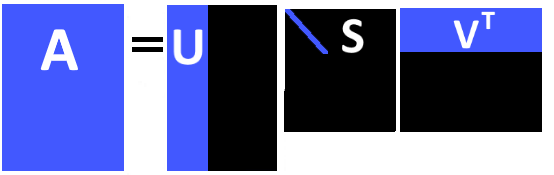
\includegraphics[width=0.7\textwidth]{figures/appendix-SVD/low_rank_decomposition_diagram}
\decoRule
\caption{Decomposition of input matrix $\mtrx{A}$ into diagonal matrix of singular values $\mtrx{S}$ and matrices of left and right singular vectors. Light color illustrates low-rank approximation.}
\label{fig:lowrank_svd}
\end{figure}

%----------------------------------------------------------------------------------------
%	SUB-SECTION Error estimation
%----------------------------------------------------------------------------------------

\subsection{Error estimation}
\label{sec:error-estimation}

The objective of data compression is to represent an input with smaller amount of data. However, the data reconstructed from its compressed representation may or may not be the exact copy of the original image. A compression technique can be lossy or lossless based on the quality of data it restores.

Low-rank approximation matrix method that is described in this paper is a lossy compression technique. Several error metrics are used to control the quality of results \cite{SairaBanu2015}.

\begin{itemize}
\item \textbf{Mean square error}
\begin{equation}
\mathit{MSE}=\frac{1}{m n} \sum_{i=1}^{m} \sum_{j=1}^{n} (a_{ij} - a'_{ij})^{2},
\label{eq:mse-def}
\end{equation}

\noindent
where $a_{ij}$ represents an element of the original matrix and $a'_{ij}$ represents an element of the
reconstructed matrix of dimension $m \times n$.

\item \textbf{Rooted Mean Square Deviation}
\begin{equation}
\mathit{RMSD} = \sqrt{\mathit{MSE}}.
\label{eq:rmsd-def}
\end{equation}

\item \textbf{Normalized Rooted Mean Square Deviation}
\begin{equation}
\mathit{NRMSD} = \frac{\mathit{RMSD}}{X_{max}-X_{min}}=\frac{\sqrt{\mathit{MSE}}}{X_{max}-X_{min}},
\label{eq:nrmsd-def}
\end{equation}

\noindent
where $X_{min}$ and $X_{max}$ are elements of input matrix $\mtrx{A}$ with minimum and maximum value, respectively. This error metric is able to measure and compare errors in datasets with different scales. Therefore, it is the main parameter that is used to control the quality of compression in the algorithm presented in this paper.

\item \textbf{Peak Signal to Noise Ratio}

$\mathit{PSNR}$ is most commonly used to measure the quality of reconstruction of lossy compression methods (e.g. image compression). The signal in this case is the original data, and the noise is the error introduced by compression. $\mathit{PSNR}$ is an approximation to human perception of reconstruction quality. This metric is not so important in area of FEM analyses, where the human perception of visualizations is not as important as the exact mathematical accuracy of approximations. The reason to include $\mathit{PSNR}$ in results is in particular to allow comparison with other image-related compression methods. $\mathit{PSNR}$ is usually expressed in terms of the logarithmic decibel scale (dB)

\begin{eqnarray}
\mathit{PSNR} &=& 10\log_{10}\frac{(X_{max}-X_{min})^{2}}{\mathit{MSE}} =
\\
&=& 20\log_{10}\frac{X_{max}-X_{min}}{\sqrt{\mathit{MSE}}}=20\log_{10}\frac{1}{\mathit{NRMSD}} = \nonumber
\\
&=& -20\log_{10}\mathit{NRMSD}. \nonumber
\label{eq:psnr-def}
\end{eqnarray}

\end{itemize}

%----------------------------------------------------------------------------------------
%	SUB-SECTION Randomized SVD
%----------------------------------------------------------------------------------------

\subsection{Randomized SVD}

The exact SVD of a $m \times n$ matrix has computational complexity \newline $\mathrm{O}(\mathrm{min}(mn^2, m^2n))$ using the ``big-O'' notation. When applied on large data sets it tends to be very time-consuming. In \cite{Candes2011, Woolfe2008, Martinsson2011, Szlam2014} are described randomized methods for constructing approximate matrix factorizations which offer significant speedups over classical methods.

The particular implementation of the randomized decomposition is based on the algorithm described in \cite{Halko2011}. The authors proposed an algorithm for efficient computation of low-rank approximation to a given matrix. The algorithm can be split into two main computational stages.

The first stage is to construct a low-dimensional subspace that captures the action of the matrix. To be more formal, this stage is to compute an approximate basis for the range of the input matrix $\mtrx{A}$. This basis matrix $\mtrx{Q}$ is required to have orthonormal columns and

\begin{equation}
\mtrx{A} \approx \mtrx{Q} \mtrx{Q}^{\mathsf{T}} \mtrx{A}.
\end{equation}

\noindent
Matrix $\mtrx{Q}$ is desired to contain as few columns as possible while producing accurate approximation of matrix $\mtrx{A}$ at the same time.

The second stage is to use $\mtrx{Q}$ to obtain approximate SVD factorization of $\mtrx{A}$. This can be achieved using simple deterministic steps:

\begin{enumerate}
\item Construct $\mtrx{B} = \mtrx{Q}^{\mathsf{T}} \mtrx{A}$.
\item Compute an exact SVD of the small matrix: $\mtrx{B}=\mtrx{W}\mtrx{\widetilde{S}}\mtrx{\widetilde{V}}^{\mathsf{T}}$.
\item Set $\mtrx{\widetilde{U}}=\mtrx{Q}\mtrx{W}$.
\end{enumerate}

The main challenge is therefore to efficiently construct $r$ orthonormal vectors forming the matrix $\mtrx{Q}$ that (nearly) span the range of $\mtrx{A}$; $r$ is the desired rank of approximation and is supposed to be substantially less then both dimensions of $\mtrx{A}$. After that an SVD that closely approximates $\mtrx{A}$ can be constructed (closely in the sense that the spectral norm of the difference between $\mtrx{A}$ and the approximation to $\mtrx{A}$ is small relative to the spectral norm of $\mtrx{A}$).

In order to estimate the range of matrix $\mtrx{A}$, it is applied to a collection of $r$ random vectors. The result of applying $\mtrx{A}$ to any vector is a vector in the range of $\mtrx{A}$, and if the matrix is applied to $r$ random vectors, the results will nearly span the range of $\mtrx{A}$ with extremely high probability. Mathematical proofs given in \cite{Halko2011} and \cite{Witten2015} show that the probability of missing a substantial part of the range of $\mtrx{A}$ is negligible if the vectors to which we apply $\mtrx{A}$ are sufficiently random (i.e. entries of these vectors are independent and identically distributed).

Therefore, the matrix $\mtrx{A}$ is applied to a random Gaussian matrix $\mtrx{\Omega}$ that contains $r$ columns with random normally distributed entries yielding the matrix $\mtrx{Y} = \mtrx{A} \mtrx{\Omega}$. Applying the Gram-Schmidt process (or any other method for constructing QR decomposition) produces the decomposition $\mtrx{Y}=\mtrx{Q}\mtrx{R}$, where columns of $\mtrx{Q}$ are an orthonormal basis for the range of $\mtrx{Y}$, and since columns of $\mtrx{Y}$ nearly span the range of $\mtrx{A}$, $\mtrx{Q}$ is an orthonormal basis for the approximate range of $\mtrx{A}$.

$\mtrx{A}$ is then decomposed as
\begin{equation}
\mtrx{A} \approx \mtrx{Q}\mtrx{Q}^{\mathsf{T}}\mtrx{A} = \mtrx{Q}\mtrx{B} = \mtrx{Q}\mtrx{W}\mtrx{\widetilde{S}}\mtrx{\widetilde{V}}^{\mathsf{T}} = \mtrx{\widetilde{U}}\mtrx{\widetilde{S}}\mtrx{\widetilde{V}}^{\mathsf{T}}.
\end{equation}

\noindent
The algorithm produces matrices $\mtrx{\widetilde{U}}$ and $\mtrx{\widetilde{V}}$ with orthonormal columns being approximations of left and right singular vectors of matrix $\mtrx{A}$, and a nonnegative, diagonal matrix $\mtrx{\widetilde{S}}$ that contains approximations of the first $r$ singular values of matrix $\mtrx{A}$. For a dense input matrix, randomized SVD decomposition algorithm requires $\mathrm{O}(mn \log{k})$ floating-point operations, substantially less than classical algorithms.

%----------------------------------------------------------------------------------------
%	SECTION Implementation
%----------------------------------------------------------------------------------------

\section{Implementation}

SVD decomposition is applied on matrices. The first thing to do is therefore to assemble an input matrix. Results from the finite element method are scalar, vector, or tensor fields represented by discrete values calculated in nodes of the mesh or in integration points on finite elements. As an example can serve temperature field, vector of nodal displacements, strain tensor evaluated in integration points, etc. There are two similar sets of results. One is generated by a non-linear algorithms, where several incremental steps are stored and the other is generated by time integration, where results in particular time steps are stored. In order to compress data, an auxiliary matrix $\mtrx{A}$ has to be assembled. The number of rows of the matrix $\mtrx{A}$ is equal to the number of incremental or time steps while the number of columns is equal to the number of points in which the results are stored. Such auxiliary matrix is assembled for each scalar field and for each component of the vector and tensor fields. It means, three matrices corresponding to the displacement in the $x$, $y$ and $z$ directions are assembled for the vector of displacements in three-dimensional problems.

There are two main reasons to store particular results in separate matrices. First, the size of matrices is smaller than the size of a matrix which contains all results and therefore the SVD will be performed faster. Second, the magnitudes of particular fields are very different (the stress tensor components are several order of magnitude larger than the components of the displacement vector) and the data compression algorithm would suppress the fields with small magnitudes. Once the matrices $\mtrx{A}$ are assembled for each field, the compression algorithm can be applied on it. It is purely algebraic procedure and no information about geometry of the mesh is needed.

Let us assume that the matrix is not empty and is full rank. Then from the formula (\ref{eq:cr-def}) follows that if $r$ equals to the rank of matrix $\mtrx{A}$ the compression ratio is always higher than one. In other words the memory consumption of stored decomposition is bigger than the size of the original matrix. To make the compression algorithm applicable the parameter $r$ must satisfy the condition

\begin{equation}
r<\frac{m n}{m+n+1}.
\label{eq:r-ineq}
\end{equation}

\noindent
Considering the usual shape of matrix containing FEM results this inequality is easily satisfiable even for the $r$ being close to the rank of the original matrix as in the typical case the number of nodes or integration points is much higher than the number of analysis steps and therefore $m \ll n$.

%----------------------------------------------------------------------------------------
%	SUB-SECTION Algorithm description
%----------------------------------------------------------------------------------------

\subsection{Algorithm description}
Once the SVD decomposition is calculated the compression algorithm removes a certain number of singular values and corresponding singular vectors. The remaining singular values and vectors represent the compressed data. There are two strategies that influence the way how to get the number of singular values to be preserved -- resulting size and quality. Each strategy is assigned a control parameter that determines compression ratio or approximation error.

\paragraph{Compression ratio}
If the focus is only on the size of compressed data, the rank $r$ of the approximation matrix can be calculated by the formula

\begin{equation}
r=\ceil*{c \times \frac{m n}{m+n+1}},
\label{eq:rank-from-comp-ratio}
\end{equation}

\noindent
where $c$ is the compression ratio, $0 \leq c \leq 1$ ($0$ results in absolute compression while $1$ results in no compression); $\ceil*{.}$ is the ceiling function.

\paragraph{Approximation error}
In the usual case the most important measure to take into account is the approximation error. Algorithm is trying to minimize the compression ratio while at the same time ensuring that predefined approximation error threshold is not exceeded. To quantify the error the Normalized root-mean-square deviation ($\mathit{NRMSD}$) is used. The normalized error metric enables to work with various data sets that have different scales. $\mathit{NRMSD}$ is defined in section \ref{sec:error-estimation}.

To effectively calculate the final rank of the approximation matrix from the desired approximation error the interesting property of singular values

% TODO: Reference to source or further explanation needed. (prof. Marek?)

\begin{equation}
\sum_{i=1}^{m} \sum_{j=1}^{n} (a_{ij})^{2} = \sum_{i=1}^{k}{s_{i}^{2}},
\label{eq:elem-sqr-sigma-sqr}
\end{equation}

\noindent
where $k=min(m, n)$, i.e. the smallest of two dimensions of the matrix $\mtrx{A}$, is made use of. The above formula states that the sum of squared elements of matrix $\mtrx{A}$ equals to the sum of squared singular values $s_{i}$ of the same matrix $\mtrx{A}$.

Using formulas \eqref{eq:svd-expansion} and \eqref{eq:svd-approx-expansion} the equation \eqref{eq:elem-sqr-sigma-sqr} can be applied to the difference between original matrix $\mtrx{A}$ and approximation matrix $\mtrx{A'}$

\begin{equation}
\sum_{i=1}^{m} \sum_{j=1}^{n} (a_{ij} - a'_{ij})^{2} = \sum_{i=r+1}^{k}{s_{i}^{2}},
\end{equation}

\noindent
where the term on the right-hand side is the sum of squares of those singular values of the matrix $\mtrx{A}$ that are going to be cut away by the compression algorithm. The equation can be rewritten using the definition of $\mathit{MSE}$ in \eqref{eq:mse-def} to

\begin{equation}
%MSE \times m n = s_{r+1}^{2} + s_{r+2}^{2} + ... + s_{k-1}^{2} + s_{k}^2
\mathit{MSE} \times m n = \sum_{i=r+1}^{k} s_{i}^{2}
\end{equation}

\noindent
and using \eqref{eq:nrmsd-def} further to

\begin{equation}
%(NRMSD \times (X_{max}-X_{min}))^{2} \times m n = s_{r+1}^{2} + s_{r+2}^{2} + ... + s_{k-1}^{2} + s_{k}^2.
(\mathit{NRMSD} \times (X_{max}-X_{min}))^{2} \times m n = \sum_{i=r+1}^{k} s_{i}^{2}.
\end{equation}

Then $\mathit{NRMSD}$ can be used as a quality metric for the compression algorithm because normalization makes it usable for different datasets. Calculation of rank of the approximation matrix is depicted as pseudo-code in Algorithm \ref{alg:rank-calculation}. Algorithm uses the inequality

\begin{equation}
e > \frac{\sqrt[]{\frac{\sum_{i=r+1}^{k} s_{i}^{2}}{m n}}}{X_{max}-X_{min}},
\end{equation}

\noindent
to test whether the desired rank has been reached; $e$ is $\mathit{NRMSD}$ used as an error threshold that can not be exceeded to achieve reasonable quality of approximation.

\begin{algorithm}
  \caption{Calculation of rank for approximation matrix from maximum allowed error}\label{rankAlgorithm}
  \label{alg:rank-calculation}
  \begin{algorithmic}[1]
  	\INPUT maximum allowed error ($e$), array with singular values ($S$), element count ($c$), maximum element value ($x_{max}$), minimum element value ($x_{min}$)
    \OUTPUT rank of resulting matrix
    \Procedure{CalculateRank}{$e, S, c, x_{max}, x_{min}$}
      \State $\mathit{MSE} \gets 0$
      \State $\mathit{NRMSD} \gets 0$
      \State $rank \gets S.length$
      \While{$\mathit{NRMSD} < e$}\Comment{repeat until max error is reached}
        \State $\mathit{MSE} \gets \mathit{MSE} + S[rank]/c$ \Comment{calculate $\mathit{MSE}$ for current rank}
        \State $\mathit{NRMSD} \gets \sqrt{\mathit{MSE}} / (x_{max} - x_{min})$ \Comment{normalize error}
        \State $rank \gets rank - 1$ \Comment{decrement rank for next loop}
      \EndWhile
      \State \textbf{return} $rank + 1$ \Comment{Add one to not exceed maximum allowed error}
    \EndProcedure
  \end{algorithmic}
\end{algorithm}

%----------------------------------------------------------------------------------------
%	SUB-SECTION Optimization
%----------------------------------------------------------------------------------------

\subsection{Optimization}

% http://mathoverflow.net/questions/161252/what-is-the-time-complexity-of-truncated-svd

Computational complexity of the exact SVD decomposition algorithm is $\mathrm{O}(m^2n)$, where $m<n$. This theoretical algorithm complexity is confirmed by two benchmarks where the dependency of execution time on varying matrix dimension is shown. The results of the benchmarks are depicted in Figure \ref{fig:ExeTime_rows} and Figure \ref{fig:ExeTime_columns}. Several observations were made from the results:

\begin{itemize}
\item The algorithm is most efficient in cases where one dimension of the input matrix is very small compared to the other. However, this is almost always the case when compressing results from FEM -- number of incremental or time steps seldom exceeds hundreds.
\item Moreover, incremental or time steps can be split into smaller ranges and the algorithm can be applied on each range separately. This will improve performance and can also increase quality of compression if the key time steps on the range boundaries are carefully selected.
\item Randomized SVD algorithm has the same order of algorithmic complexity when full decomposition is required, but yet can significantly reduce execution time. However, the benchmarks are not designed to highlight the benefits of randomized SVD algorithms. The main advantage of the randomized SVD is in the ability to choose the rank of the approximation matrix in advance. In that case only limited number of singular values and corresponding singular vectors is calculated and algorithm performs much faster.
\end{itemize}

Storage size of SVD decomposition itself can also be optimized. $\mtrx{S}$ being a diagonal matrix can be stored as single list of singular values $s_{i}$ or can be even multiplied with the matrix of left singular vectors $\mtrx{U}$.

% main features for optimization: key time steps (time step span compression), Randomized SVD, Parallelization, Sparse matrix of details, prenasobeni U matice singularnimi cisly, trochu usetrim pamet, mohu pouzit vzorkovani...

%----------------------------------------------------------------------------------------
%	SECTION Results
%----------------------------------------------------------------------------------------

\section{Results}
\label{sec:results}

The number of operations in the compression algorithm with respect to the number of stored incremental or time steps (the number of rows in the matrix $\mtrx{A}$) is depicted in Figure \ref{fig:ExeTime_rows} while the number of operations with respect to the number of points, where the results are stored (the number of columns of the matrix $\mtrx{A}$), is depicted in Figure \ref{fig:ExeTime_columns}. Especially on Figure \ref{fig:ExeTime_columns} is clearly visible that the randomized SVD algorithm is much faster than the classical one.

These results confirm that the SVD implementation has computational complexity $\mathrm{O}(m^2n)$, where $m$ is number of rows, $n$ is number of columns, and $m < n$. In case of $m > n$ the complexity would be $\mathrm{O}(mn^2)$ as the algorithm takes advantage of non-squareness in that its complexity is only linear in the greater dimension.

\begin{figure}[H]
\centering
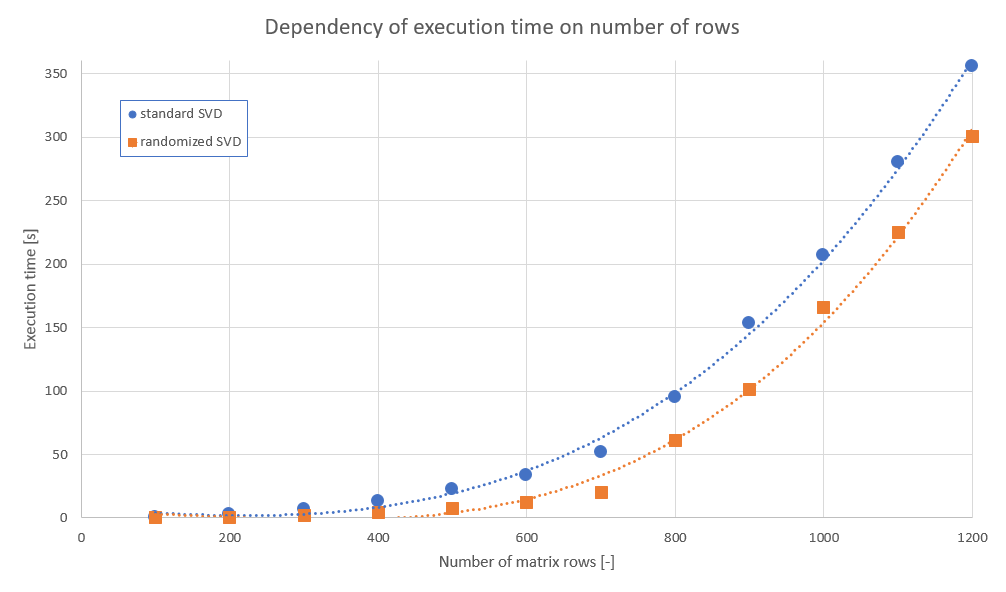
\includegraphics[width=\textwidth]{figures/appendix-SVD/executionTime_varyingRows}
\decoRule
\caption{Dependency of SVD execution time on number of rows of an input matrix (having fixed number of columns).}
\label{fig:ExeTime_rows}
\end{figure}

\begin{figure}[H]
\centering
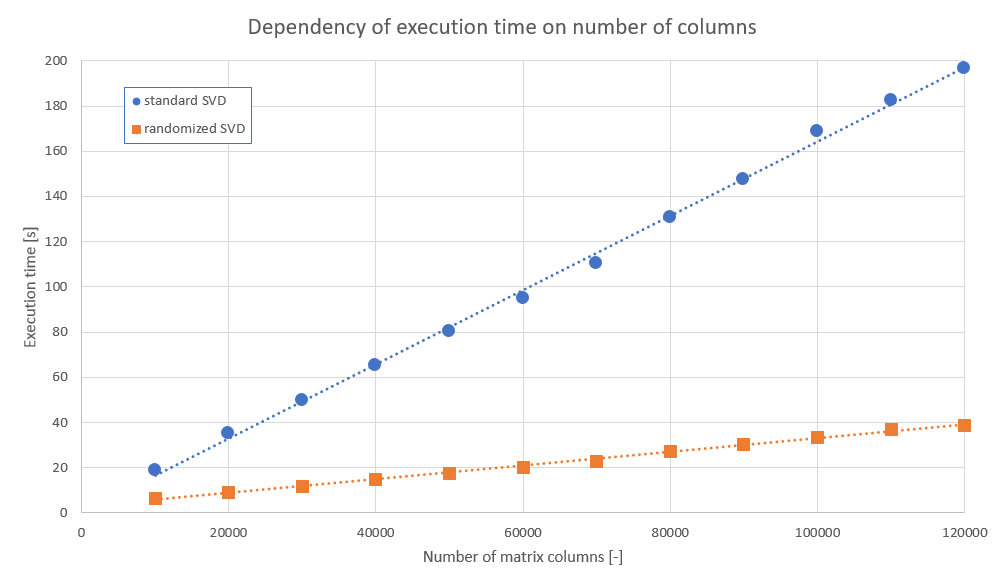
\includegraphics[width=\textwidth]{figures/appendix-SVD/executionTime_varyingColumns}
\decoRule
\caption{Dependency of SVD execution time on number of columns of an input matrix (having fixed number of rows).}
\label{fig:ExeTime_columns}
\end{figure}

% reactor containment
Behavior of the compression strategy introduced is presented on three real world examples. First example is an analysis of aging of nuclear power plant's containment made from prestressed concrete. Finite element mesh used in this analysis is in Figure \ref{fig:temelin:mesh}. More details about the analysis can be found in \cite{Kruis2012} and \cite{Koudelka2009}. This analysis includes high number of analysis time steps (thousands) with very little differences between them. There is therefore potential for compression ratio to be very high as proven in Figure \ref{fig:temelin:NRMSD} that examines the impact of changes in the compression ratio to the mean error of approximation.

\begin{figure}[H]
\centering
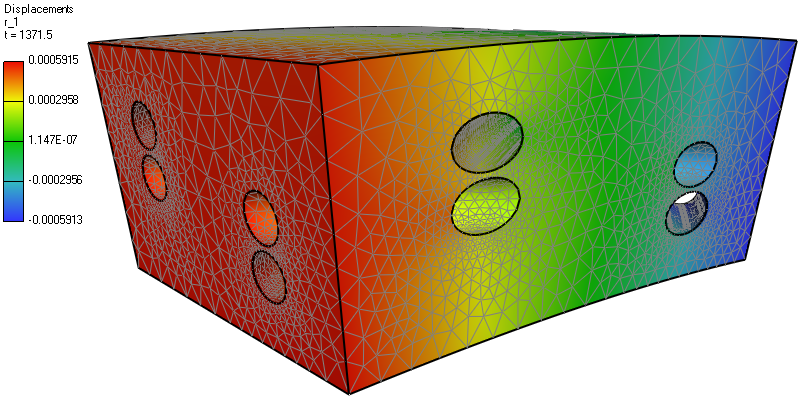
\includegraphics[width=\textwidth]{figures/appendix-SVD/temelin_screenshot}
\decoRule
\caption{Segment of containment analyzed. Results visualization (displacement field, x component).}
\label{fig:temelin:mesh}
\end{figure}

\begin{figure}[H]
\centering
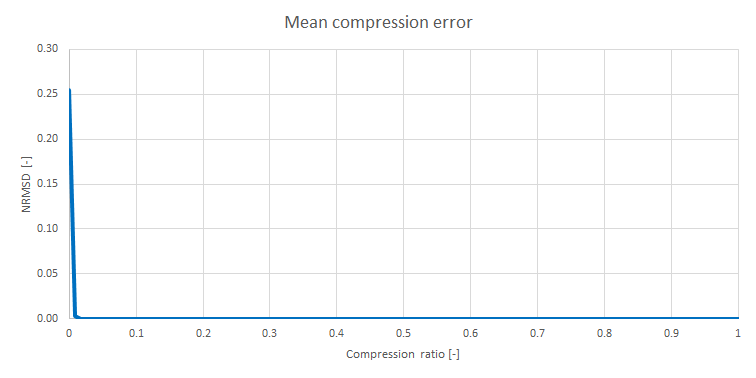
\includegraphics[width=\textwidth]{figures/appendix-SVD/temelin_NRMSD}
\decoRule
\caption{Dependence of Normalized Rooted Mean Squared Deviation on Compression ratio for reactor containment analysis results.}
\label{fig:temelin:NRMSD}
\end{figure}

% geological layers
Figure \ref{fig:chotkova:mesh}  shows results from an analysis of geological layers which was based on theory plasticity. More details can be found in \cite{Koudelka2006}. This project was chosen mainly to study behavior of compression algorithm when dealing with high discontinuities in data in spatial dimension (as can be seen in visualization). As summarized in Figure \ref{fig:chotkova:NRMSD} and Figure \ref{fig:chotkova:MaxError} this has negligible effect on quality of compression.

\begin{figure}[H]
\centering
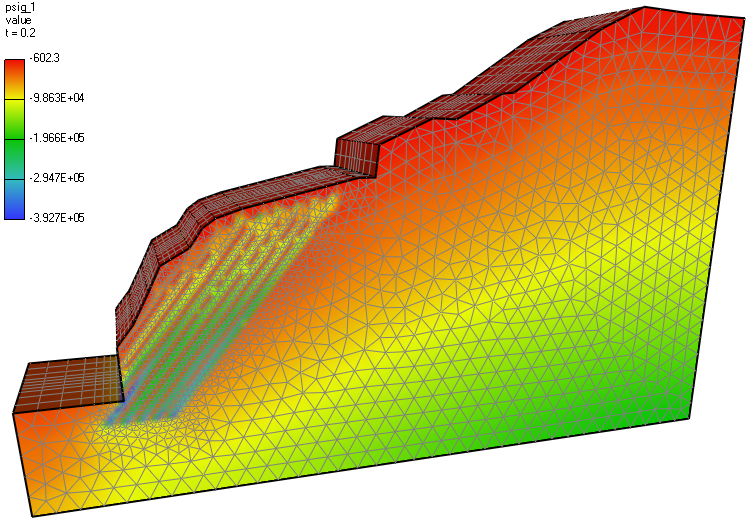
\includegraphics[width=\textwidth]{figures/appendix-SVD/chotkova_screenshot}
\decoRule
\caption{Analysis of geological layers. Results visualization (stress field, sigma XX component).}
\label{fig:chotkova:mesh}
\end{figure}

\begin{figure}[H]
\centering
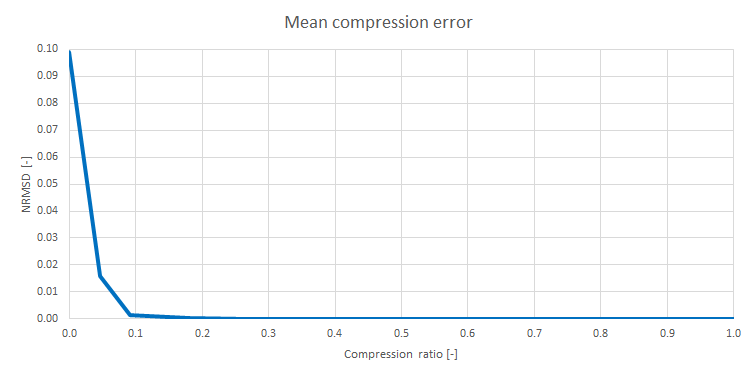
\includegraphics[width=\textwidth]{figures/appendix-SVD/chotkova_NRMSD}
\decoRule
\caption{Dependence of Normalized Rooted Mean Squared Deviation on Compression ratio for results of geological layers project.}
\label{fig:chotkova:NRMSD}
\end{figure}

\begin{figure}[H]
\centering
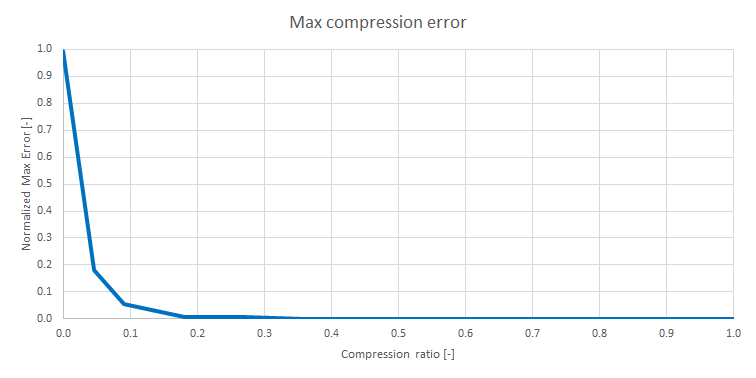
\includegraphics[width=\textwidth]{figures/appendix-SVD/chotkova_MaxError}
\decoRule
\caption{Dependence of Normalized Maximum Error on Compression ratio for results of geological layers project.}
\label{fig:chotkova:MaxError}
\end{figure}

% reactor vessel 2D
Figure \ref{fig:mechaxisym:mesh} contains visualization of results of two-dimensional analysis, where axisymmetric description was used for analysis of aging of a reactor vessel. Details about the analysis can be found in \cite{Kruis2005}. There are exactly 232 analysis time steps. The resulting data has linear function character with several discontinuities in temporal dimension. There are few time steps in which resulting discrete functions have very different values compared to neighboring time steps. This was supposed to have negative impact on the quality of compression. However, as can be seen in Figure \ref{fig:mechaxisym:NRMSD}, the quality is better than expected; e.g., if the rank of approximation matrix is set to 3 (compared to 232 being the rank of the original matrix) the normalized relative error ($\mathit{NRMSD}$) does not exceed $10^{-5}$.

\begin{figure}[H]
\centering
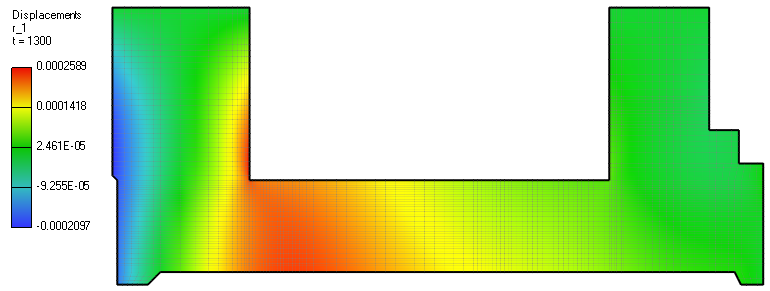
\includegraphics[width=\textwidth]{figures/appendix-SVD/mechaxisym_screenshot}
\decoRule
\caption{2D model of a reactor vessel. Results visualization (displacement field, x component).}
\label{fig:mechaxisym:mesh}
\end{figure}

\begin{figure}[H]
\centering
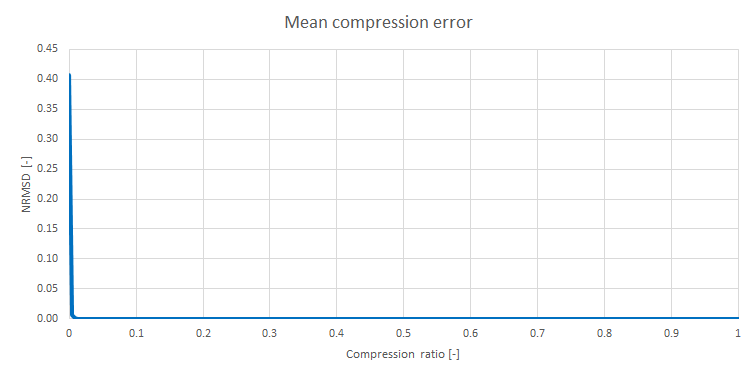
\includegraphics[width=\textwidth]{figures/appendix-SVD/mechaxisym_NRMSD}
\decoRule
\caption{Dependence of Normalized Rooted Mean Squared Deviation on Compression ratio for reactor vessel analysis results.}
\label{fig:mechaxisym:NRMSD}
\end{figure}

% PSNR
Figure \ref{fig:PSNR} summarizes the compression error for all three benchmarks using logarithmic scale to make the differences more visible. Peek signal to noise ratio ($\mathit{PSNR}$) metric is used (see Equation \ref{eq:psnr-def} for definition). Figure \ref{fig:PSNR_rand} contains the same comparison for the randomized SVD algorithm.

\begin{figure}[H]
\centering
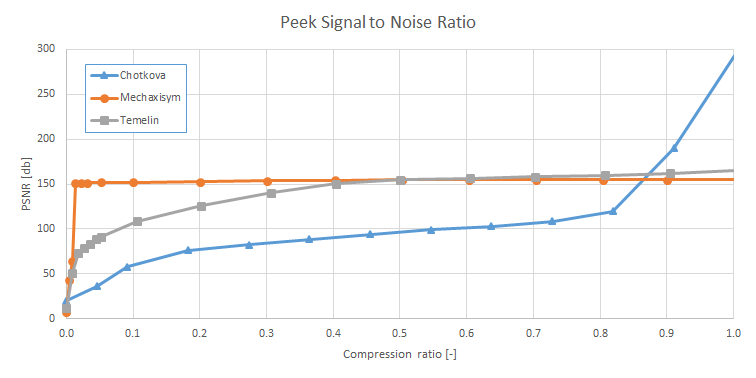
\includegraphics[width=\textwidth]{figures/appendix-SVD/PSNR}
\decoRule
\caption{Comparison of Peek signal to noise ratio value calculated for different decompositions.}
\label{fig:PSNR}
\end{figure}

\begin{figure}[H]
\centering
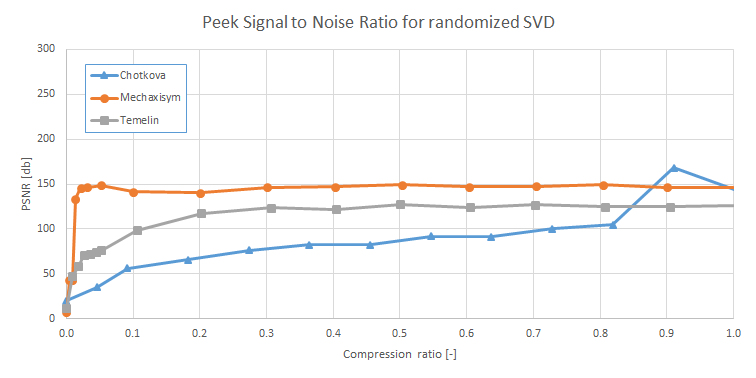
\includegraphics[width=\textwidth]{figures/appendix-SVD/PSNR_rand}
\decoRule
\caption{Comparison of Peek signal to noise ratio value for different randomized decompositions.}
\label{fig:PSNR_rand}
\end{figure}

% Execution times
Besides the error also the execution speed of compression algorithm was measured. In Figure \ref{fig:temelin:ExeTime} is comparison of execution times for standard versus randomized SVD compression algorithms. Interestingly, execution time of standard SVD is independent of target rank whereas execution time of randomized SVD decreases linearly with decreasing target rank. If the rank is known ahead of time the fact can be taken advantage of.

\begin{figure}[H]
\centering
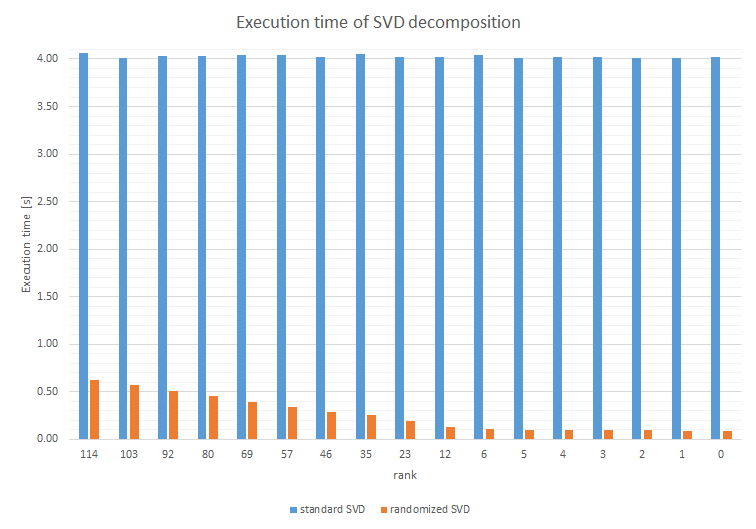
\includegraphics[width=\textwidth]{figures/appendix-SVD/temelin_ExecutionTime}
\decoRule
\caption{Variation of execution time of standard and randomized decompositions calculated for reactor containment analysis results.}
\label{fig:temelin:ExeTime}
\end{figure}

The memory consumption of compressed results for reactor containment analysis is summarized in Table \ref{tab:mem-consum}. For different values of compression ratio shows memory size in megabytes. Compression ratio $c$ is an input parameter to the compression algorithm specifying amount of singular values ought to be removed from the SVD decomposition as follows from the equation (\ref{eq:rank-from-comp-ratio}). Size factor describes the final outcome of compression when compared to the original size.

\begin{table}[H]
\centering
\caption[Memory consumption of SVD compression]{Memory consumption of compressed results. 3D reactor containment analysis.}
    \begin{tabular}{|r | r | r|}
    \hline
    compression ratio ($c$) & memory consumption [MB] & size factor \\ \hline
    1.00 & 2002.1 & 1 \\
    0.50 & 1006.9 & 0.5002 \\
    0.10& 211.9 & 0.1053 \\
    0.01 & 35.3 & 0.0176 \\ \hline
    \end{tabular}
	\label{tab:mem-consum}
\end{table}

\chapter{Data format for storage and transport of FEM-related data}
\label{appendix-data-format}

% Examples of solution.json, summary.json, mesh.json, attribute.json, and result.json files
% TODO: remove this Appendix

\chapter{How to write thesis in TeX} % Main chapter title

\label{Chapter1} % For referencing the chapter elsewhere, use \ref{Chapter1} 

%----------------------------------------------------------------------------------------

% Define some commands to keep the formatting separated from the content 
\newcommand{\keyword}[1]{\textbf{#1}}
%\newcommand{\tabhead}[1]{\textbf{#1}}
\newcommand{\code}[1]{\texttt{#1}}
\newcommand{\file}[1]{\texttt{\bfseries#1}}
\newcommand{\option}[1]{\texttt{\itshape#1}}

%----------------------------------------------------------------------------------------

\section{Welcome and Thank You}
Welcome to this \LaTeX{} Thesis Template, a beautiful and easy to use template for writing a thesis using the \LaTeX{} typesetting system.

If you are writing a thesis (or will be in the future) and its subject is technical or mathematical (though it doesn't have to be), then creating it in \LaTeX{} is highly recommended as a way to make sure you can just get down to the essential writing without having to worry over formatting or wasting time arguing with your word processor.

\LaTeX{} is easily able to professionally typeset documents that run to hundreds or thousands of pages long. With simple mark-up commands, it automatically sets out the table of contents, margins, page headers and footers and keeps the formatting consistent and beautiful. One of its main strengths is the way it can easily typeset mathematics, even \emph{heavy} mathematics. Even if those equations are the most horribly twisted and most difficult mathematical problems that can only be solved on a super-computer, you can at least count on \LaTeX{} to make them look stunning.

%----------------------------------------------------------------------------------------

\section{Learning \LaTeX{}}

\LaTeX{} is not a \textsc{wysiwyg} (What You See is What You Get) program, unlike word processors such as Microsoft Word or Apple's Pages. Instead, a document written for \LaTeX{} is actually a simple, plain text file that contains \emph{no formatting}. You tell \LaTeX{} how you want the formatting in the finished document by writing in simple commands amongst the text, for example, if I want to use \emph{italic text for emphasis}, I write the \verb|\emph{text}| command and put the text I want in italics in between the curly braces. This means that \LaTeX{} is a \enquote{mark-up} language, very much like HTML.

\subsection{A (not so short) Introduction to \LaTeX{}}

If you are new to \LaTeX{}, there is a very good eBook -- freely available online as a PDF file -- called, \enquote{The Not So Short Introduction to \LaTeX{}}. The book's title is typically shortened to just \emph{lshort}. You can download the latest version (as it is occasionally updated) from here:
\url{http://www.ctan.org/tex-archive/info/lshort/english/lshort.pdf}

It is also available in several other languages. Find yours from the list on this page: \url{http://www.ctan.org/tex-archive/info/lshort/}

It is recommended to take a little time out to learn how to use \LaTeX{} by creating several, small `test' documents, or having a close look at several templates on:\\ 
\url{http://www.LaTeXTemplates.com}\\ 
Making the effort now means you're not stuck learning the system when what you \emph{really} need to be doing is writing your thesis.

\subsection{A Short Math Guide for \LaTeX{}}

If you are writing a technical or mathematical thesis, then you may want to read the document by the AMS (American Mathematical Society) called, \enquote{A Short Math Guide for \LaTeX{}}. It can be found online here:
\url{http://www.ams.org/tex/amslatex.html}
under the \enquote{Additional Documentation} section towards the bottom of the page.

\subsection{Common \LaTeX{} Math Symbols}
There are a multitude of mathematical symbols available for \LaTeX{} and it would take a great effort to learn the commands for them all. The most common ones you are likely to use are shown on this page:
\url{http://www.sunilpatel.co.uk/latex-type/latex-math-symbols/}

You can use this page as a reference or crib sheet, the symbols are rendered as large, high quality images so you can quickly find the \LaTeX{} command for the symbol you need.

\subsection{\LaTeX{} on a Mac}
 
The \LaTeX{} distribution is available for many systems including Windows, Linux and Mac OS X. The package for OS X is called MacTeX and it contains all the applications you need -- bundled together and pre-customized -- for a fully working \LaTeX{} environment and work flow.
 
MacTeX includes a custom dedicated \LaTeX{} editor called TeXShop for writing your `\file{.tex}' files and BibDesk: a program to manage your references and create your bibliography section just as easily as managing songs and creating playlists in iTunes.

%----------------------------------------------------------------------------------------

\section{Getting Started with this Template}

If you are familiar with \LaTeX{}, then you should explore the directory structure of the template and then proceed to place your own information into the \emph{THESIS INFORMATION} block of the \file{main.tex} file. You can then modify the rest of this file to your unique specifications based on your degree/university. Section \ref{FillingFile} on page \pageref{FillingFile} will help you do this. Make sure you also read section \ref{ThesisConventions} about thesis conventions to get the most out of this template.

If you are new to \LaTeX{} it is recommended that you carry on reading through the rest of the information in this document.

Before you begin using this template you should ensure that its style complies with the thesis style guidelines imposed by your institution. In most cases this template style and layout will be suitable. If it is not, it may only require a small change to bring the template in line with your institution's recommendations. These modifications will need to be done on the \file{MastersDoctoralThesis.cls} file.

\subsection{About this Template}

This \LaTeX{} Thesis Template is originally based and created around a \LaTeX{} style file created by Steve R.\ Gunn from the University of Southampton (UK), department of Electronics and Computer Science. You can find his original thesis style file at his site, here:
\url{http://www.ecs.soton.ac.uk/~srg/softwaretools/document/templates/}

Steve's \file{ecsthesis.cls} was then taken by Sunil Patel who modified it by creating a skeleton framework and folder structure to place the thesis files in. The resulting template can be found on Sunil's site here:
\url{http://www.sunilpatel.co.uk/thesis-template}

Sunil's template was made available through \url{http://www.LaTeXTemplates.com} where it was modified many times based on user requests and questions. Version 2.0 and onwards of this template represents a major modification to Sunil's template and is, in fact, hardly recognisable. The work to make version 2.0 possible was carried out by \href{mailto:vel@latextemplates.com}{Vel} and Johannes Böttcher.

%----------------------------------------------------------------------------------------

\section{What this Template Includes}

\subsection{Folders}

This template comes as a single zip file that expands out to several files and folders. The folder names are mostly self-explanatory:

\keyword{Appendices} -- this is the folder where you put the appendices. Each appendix should go into its own separate \file{.tex} file. An example and template are included in the directory.

\keyword{Chapters} -- this is the folder where you put the thesis chapters. A thesis usually has about six chapters, though there is no hard rule on this. Each chapter should go in its own separate \file{.tex} file and they can be split as:
\begin{itemize}
\item Chapter 1: Introduction to the thesis topic
\item Chapter 2: Background information and theory
\item Chapter 3: (Laboratory) experimental setup
\item Chapter 4: Details of experiment 1
\item Chapter 5: Details of experiment 2
\item Chapter 6: Discussion of the experimental results
\item Chapter 7: Conclusion and future directions
\end{itemize}
This chapter layout is specialised for the experimental sciences, your discipline may be different.

\keyword{Figures} -- this folder contains all figures for the thesis. These are the final images that will go into the thesis document.

\subsection{Files}

Included are also several files, most of them are plain text and you can see their contents in a text editor. After initial compilation, you will see that more auxiliary files are created by \LaTeX{} or BibTeX and which you don't need to delete or worry about:

\keyword{example.bib} -- this is an important file that contains all the bibliographic information and references that you will be citing in the thesis for use with BibTeX. You can write it manually, but there are reference manager programs available that will create and manage it for you. Bibliographies in \LaTeX{} are a large subject and you may need to read about BibTeX before starting with this. Many modern reference managers will allow you to export your references in BibTeX format which greatly eases the amount of work you have to do.

\keyword{MastersDoctoralThesis.cls} -- this is an important file. It is the class file that tells \LaTeX{} how to format the thesis. 

\keyword{main.pdf} -- this is your beautifully typeset thesis (in the PDF file format) created by \LaTeX{}. It is supplied in the PDF with the template and after you compile the template you should get an identical version.

\keyword{main.tex} -- this is an important file. This is the file that you tell \LaTeX{} to compile to produce your thesis as a PDF file. It contains the framework and constructs that tell \LaTeX{} how to layout the thesis. It is heavily commented so you can read exactly what each line of code does and why it is there. After you put your own information into the \emph{THESIS INFORMATION} block -- you have now started your thesis!

Files that are \emph{not} included, but are created by \LaTeX{} as auxiliary files include:

\keyword{main.aux} -- this is an auxiliary file generated by \LaTeX{}, if it is deleted \LaTeX{} simply regenerates it when you run the main \file{.tex} file.

\keyword{main.bbl} -- this is an auxiliary file generated by BibTeX, if it is deleted, BibTeX simply regenerates it when you run the \file{main.aux} file. Whereas the \file{.bib} file contains all the references you have, this \file{.bbl} file contains the references you have actually cited in the thesis and is used to build the bibliography section of the thesis.

\keyword{main.blg} -- this is an auxiliary file generated by BibTeX, if it is deleted BibTeX simply regenerates it when you run the main \file{.aux} file.

\keyword{main.lof} -- this is an auxiliary file generated by \LaTeX{}, if it is deleted \LaTeX{} simply regenerates it when you run the main \file{.tex} file. It tells \LaTeX{} how to build the \emph{List of Figures} section.

\keyword{main.log} -- this is an auxiliary file generated by \LaTeX{}, if it is deleted \LaTeX{} simply regenerates it when you run the main \file{.tex} file. It contains messages from \LaTeX{}, if you receive errors and warnings from \LaTeX{}, they will be in this \file{.log} file.

\keyword{main.lot} -- this is an auxiliary file generated by \LaTeX{}, if it is deleted \LaTeX{} simply regenerates it when you run the main \file{.tex} file. It tells \LaTeX{} how to build the \emph{List of Tables} section.

\keyword{main.out} -- this is an auxiliary file generated by \LaTeX{}, if it is deleted \LaTeX{} simply regenerates it when you run the main \file{.tex} file.

So from this long list, only the files with the \file{.bib}, \file{.cls} and \file{.tex} extensions are the most important ones. The other auxiliary files can be ignored or deleted as \LaTeX{} and BibTeX will regenerate them.

%----------------------------------------------------------------------------------------

\section{Filling in Your Information in the \file{main.tex} File}\label{FillingFile}

You will need to personalise the thesis template and make it your own by filling in your own information. This is done by editing the \file{main.tex} file in a text editor or your favourite LaTeX environment.

Open the file and scroll down to the third large block titled \emph{THESIS INFORMATION} where you can see the entries for \emph{University Name}, \emph{Department Name}, etc \ldots

Fill out the information about yourself, your group and institution. You can also insert web links, if you do, make sure you use the full URL, including the \code{http://} for this. If you don't want these to be linked, simply remove the \verb|\href{url}{name}| and only leave the name.

When you have done this, save the file and recompile \code{main.tex}. All the information you filled in should now be in the PDF, complete with web links. You can now begin your thesis proper!

%----------------------------------------------------------------------------------------

\section{The \code{main.tex} File Explained}

The \file{main.tex} file contains the structure of the thesis. There are plenty of written comments that explain what pages, sections and formatting the \LaTeX{} code is creating. Each major document element is divided into commented blocks with titles in all capitals to make it obvious what the following bit of code is doing. Initially there seems to be a lot of \LaTeX{} code, but this is all formatting, and it has all been taken care of so you don't have to do it.

Begin by checking that your information on the title page is correct. For the thesis declaration, your institution may insist on something different than the text given. If this is the case, just replace what you see with what is required in the \emph{DECLARATION PAGE} block.

Then comes a page which contains a funny quote. You can put your own, or quote your favourite scientist, author, person, and so on. Make sure to put the name of the person who you took the quote from.

Following this is the abstract page which summarises your work in a condensed way and can almost be used as a standalone document to describe what you have done. The text you write will cause the heading to move up so don't worry about running out of space.

Next come the acknowledgements. On this page, write about all the people who you wish to thank (not forgetting parents, partners and your advisor/supervisor).

The contents pages, list of figures and tables are all taken care of for you and do not need to be manually created or edited. The next set of pages are more likely to be optional and can be deleted since they are for a more technical thesis: insert a list of abbreviations you have used in the thesis, then a list of the physical constants and numbers you refer to and finally, a list of mathematical symbols used in any formulae. Making the effort to fill these tables means the reader has a one-stop place to refer to instead of searching the internet and references to try and find out what you meant by certain abbreviations or symbols.

The list of symbols is split into the Roman and Greek alphabets. Whereas the abbreviations and symbols ought to be listed in alphabetical order (and this is \emph{not} done automatically for you) the list of physical constants should be grouped into similar themes.

The next page contains a one line dedication. Who will you dedicate your thesis to?

Finally, there is the block where the chapters are included. Uncomment the lines (delete the \code{\%} character) as you write the chapters. Each chapter should be written in its own file and put into the \emph{Chapters} folder and named \file{Chapter1}, \file{Chapter2}, etc\ldots Similarly for the appendices, uncomment the lines as you need them. Each appendix should go into its own file and placed in the \emph{Appendices} folder.

After the preamble, chapters and appendices finally comes the bibliography. The bibliography style (called \option{authoryear}) is used for the bibliography and is a fully featured style that will even include links to where the referenced paper can be found online. Do not underestimate how grateful your reader will be to find that a reference to a paper is just a click away. Of course, this relies on you putting the URL information into the BibTeX file in the first place.

%----------------------------------------------------------------------------------------

\section{Thesis Features and Conventions}\label{ThesisConventions}

To get the best out of this template, there are a few conventions that you may want to follow.

One of the most important (and most difficult) things to keep track of in such a long document as a thesis is consistency. Using certain conventions and ways of doing things (such as using a Todo list) makes the job easier. Of course, all of these are optional and you can adopt your own method.

\subsection{Printing Format}

This thesis template is designed for double sided printing (i.e. content on the front and back of pages) as most theses are printed and bound this way. Switching to one sided printing is as simple as uncommenting the \option{oneside} option of the \code{documentclass} command at the top of the \file{main.tex} file. You may then wish to adjust the margins to suit specifications from your institution.

The headers for the pages contain the page number on the outer side (so it is easy to flick through to the page you want) and the chapter name on the inner side.

The text is set to 11 point by default with single line spacing, again, you can tune the text size and spacing should you want or need to using the options at the very start of \file{main.tex}. The spacing can be changed similarly by replacing the \option{singlespacing} with \option{onehalfspacing} or \option{doublespacing}.

\subsection{Using US Letter Paper}

The paper size used in the template is A4, which is the standard size in Europe. If you are using this thesis template elsewhere and particularly in the United States, then you may have to change the A4 paper size to the US Letter size. This can be done in the margins settings section in \file{main.tex}.

Due to the differences in the paper size, the resulting margins may be different to what you like or require (as it is common for institutions to dictate certain margin sizes). If this is the case, then the margin sizes can be tweaked by modifying the values in the same block as where you set the paper size. Now your document should be set up for US Letter paper size with suitable margins.

\subsection{References}

The \code{biblatex} package is used to format the bibliography and inserts references such as this one \parencite{Reference1}. The options used in the \file{main.tex} file mean that the in-text citations of references are formatted with the author(s) listed with the date of the publication. Multiple references are separated by semicolons (e.g. \parencite{Reference2, Reference1}) and references with more than three authors only show the first author with \emph{et al.} indicating there are more authors (e.g. \parencite{Reference3}). This is done automatically for you. To see how you use references, have a look at the \file{Chapter1.tex} source file. Many reference managers allow you to simply drag the reference into the document as you type.

Scientific references should come \emph{before} the punctuation mark if there is one (such as a comma or period). The same goes for footnotes\footnote{Such as this footnote, here down at the bottom of the page.}. You can change this but the most important thing is to keep the convention consistent throughout the thesis. Footnotes themselves should be full, descriptive sentences (beginning with a capital letter and ending with a full stop). The APA6 states: \enquote{Footnote numbers should be superscripted, [...], following any punctuation mark except a dash.} The Chicago manual of style states: \enquote{A note number should be placed at the end of a sentence or clause. The number follows any punctuation mark except the dash, which it precedes. It follows a closing parenthesis.}

The bibliography is typeset with references listed in alphabetical order by the first author's last name. This is similar to the APA referencing style. To see how \LaTeX{} typesets the bibliography, have a look at the very end of this document (or just click on the reference number links in in-text citations).

\subsubsection{A Note on bibtex}

The bibtex backend used in the template by default does not correctly handle unicode character encoding (i.e. "international" characters). You may see a warning about this in the compilation log and, if your references contain unicode characters, they may not show up correctly or at all. The solution to this is to use the biber backend instead of the outdated bibtex backend. This is done by finding this in \file{main.tex}: \option{backend=bibtex} and changing it to \option{backend=biber}. You will then need to delete all auxiliary BibTeX files and navigate to the template directory in your terminal (command prompt). Once there, simply type \code{biber main} and biber will compile your bibliography. You can then compile \file{main.tex} as normal and your bibliography will be updated. An alternative is to set up your LaTeX editor to compile with biber instead of bibtex, see \href{http://tex.stackexchange.com/questions/154751/biblatex-with-biber-configuring-my-editor-to-avoid-undefined-citations/}{here} for how to do this for various editors.

\subsection{Tables}

Tables are an important way of displaying your results, below is an example table which was generated with this code:

{\small
\begin{verbatim}
\begin{table}
\caption{The effects of treatments X and Y on the four groups studied.}
\label{tab:treatments}
\centering
\begin{tabular}{l l l}
\toprule
\tabhead{Groups} & \tabhead{Treatment X} & \tabhead{Treatment Y} \\
\midrule
1 & 0.2 & 0.8\\
2 & 0.17 & 0.7\\
3 & 0.24 & 0.75\\
4 & 0.68 & 0.3\\
\bottomrule\\
\end{tabular}
\end{table}
\end{verbatim}
}

\begin{table}
\caption{The effects of treatments X and Y on the four groups studied.}
\label{tab:treatments}
\centering
\begin{tabular}{l l l}
\toprule
\tabhead{Groups} & \tabhead{Treatment X} & \tabhead{Treatment Y} \\
\midrule
1 & 0.2 & 0.8\\
2 & 0.17 & 0.7\\
3 & 0.24 & 0.75\\
4 & 0.68 & 0.3\\
\bottomrule\\
\end{tabular}
\end{table}

You can reference tables with \verb|\ref{<label>}| where the label is defined within the table environment. See \file{Chapter1.tex} for an example of the label and citation (e.g. Table~\ref{tab:treatments}).

\subsection{Figures}

There will hopefully be many figures in your thesis (that should be placed in the \emph{Figures} folder). The way to insert figures into your thesis is to use a code template like this:
\begin{verbatim}
\begin{figure}
\centering

\includegraphics{figures/Electron}
\decoRule
\caption[An Electron]{An electron (artist's impression).}
\label{fig:Electron}
\end{figure}
\end{verbatim}
Also look in the source file. Putting this code into the source file produces the picture of the electron that you can see in the figure below.

\begin{figure}[th]
\centering

\includegraphics{Figures/Electron}
\decoRule
\caption[An Electron]{An electron (artist's impression).}
\label{fig:Electron}
\end{figure}

Sometimes figures don't always appear where you write them in the source. The placement depends on how much space there is on the page for the figure. Sometimes there is not enough room to fit a figure directly where it should go (in relation to the text) and so \LaTeX{} puts it at the top of the next page. Positioning figures is the job of \LaTeX{} and so you should only worry about making them look good!

Figures usually should have captions just in case you need to refer to them (such as in Figure~\ref{fig:Electron}). The \verb|\caption| command contains two parts, the first part, inside the square brackets is the title that will appear in the \emph{List of Figures}, and so should be short. The second part in the curly brackets should contain the longer and more descriptive caption text.

The \verb|\decoRule| command is optional and simply puts an aesthetic horizontal line below the image. If you do this for one image, do it for all of them.

\LaTeX{} is capable of using images in pdf, jpg and png format.

\subsection{Typesetting mathematics}

If your thesis is going to contain heavy mathematical content, be sure that \LaTeX{} will make it look beautiful, even though it won't be able to solve the equations for you.

The \enquote{Not So Short Introduction to \LaTeX} (available on \href{http://www.ctan.org/tex-archive/info/lshort/english/lshort.pdf}{CTAN}) should tell you everything you need to know for most cases of typesetting mathematics. If you need more information, a much more thorough mathematical guide is available from the AMS called, \enquote{A Short Math Guide to \LaTeX} and can be downloaded from:
\url{ftp://ftp.ams.org/pub/tex/doc/amsmath/short-math-guide.pdf}

There are many different \LaTeX{} symbols to remember, luckily you can find the most common symbols in \href{http://ctan.org/pkg/comprehensive}{The Comprehensive \LaTeX~Symbol List}.

You can write an equation, which is automatically given an equation number by \LaTeX{} like this:
\begin{verbatim}
\begin{equation}
E = mc^{2}
\label{eqn:Einstein}
\end{equation}
\end{verbatim}

This will produce Einstein's famous energy-matter equivalence equation:
\begin{equation}
E = mc^{2}
\label{eqn:Einstein}
\end{equation}

All equations you write (which are not in the middle of paragraph text) are automatically given equation numbers by \LaTeX{}. If you don't want a particular equation numbered, use the unnumbered form:
\begin{verbatim}
\[ a^{2}=4 \]
\end{verbatim}

\section{How do I change the colors of links?}

The color of links can be changed to your liking using:

{\small\verb!\hypersetup{urlcolor=red}!}, or

{\small\verb!\hypersetup{citecolor=green}!}, or

{\small\verb!\hypersetup{allcolor=blue}!}.

\noindent If you want to completely hide the links, you can use:

{\small\verb!\hypersetup{allcolors=.}!}, or even better: 

{\small\verb!\hypersetup{hidelinks}!}.

\noindent If you want to have obvious links in the PDF but not the printed text, use:

{\small\verb!\hypersetup{colorlinks=false}!}.

%----------------------------------------------------------------------------------------

\section{Sectioning and Subsectioning}

You should break your thesis up into nice, bite-sized sections and subsections. \LaTeX{} automatically builds a table of Contents by looking at all the \verb|\chapter{}|, \verb|\section{}|  and \verb|\subsection{}| commands you write in the source.

The Table of Contents should only list the sections to three (3) levels. A \verb|chapter{}| is level zero (0). A \verb|\section{}| is level one (1) and so a \verb|\subsection{}| is level two (2). In your thesis it is likely that you will even use a \verb|subsubsection{}|, which is level three (3). The depth to which the Table of Contents is formatted is set within \file{MastersDoctoralThesis.cls}. If you need this changed, you can do it in \file{main.tex}.

%----------------------------------------------------------------------------------------

\section{In Closing}

You have reached the end of this mini-guide. You can now rename or overwrite this pdf file and begin writing your own \file{Chapter1.tex} and the rest of your thesis. The easy work of setting up the structure and framework has been taken care of for you. It's now your job to fill it out!

Good luck and have lots of fun!

\begin{flushright}
Guide written by ---\\
Sunil Patel: \href{http://www.sunilpatel.co.uk}{www.sunilpatel.co.uk}\\
Vel: \href{http://www.LaTeXTemplates.com}{LaTeXTemplates.com}
\end{flushright}


%----------------------------------------------------------------------------------------
%	BIBLIOGRAPHY
%----------------------------------------------------------------------------------------

\printbibliography[heading=bibintoc]

%----------------------------------------------------------------------------------------

\end{document}
